\documentclass{ximera}

\begin{document}
    \author{Wim Obbels}
    \xmtitle[Mama, kijk wat ik kan!]{Ximera Showcase}{}
    \label{xim:ximeraShowase}

Dit document bevat een overzicht van functionaliteit van Ximera. Het kan bovendien dienen als testcase, en als bron om stukjes code uit te kopiëren.

\pdfOnly{   													 % enkel in PDF
  \ifhandout
    Je gebruikt de HANDOUT PDF versie van de cursus;             % enkel in 'handout-PDF'
    
    Er bestaat ook een \textit{standaard} PDF die antwoorden en hints bevat.
  \else
    Je gebruikt de STANDAARD PDF versie van de cursus;           % enkel in 'standaard-PDF'

    Er bestaat ook een \textit{handout} PDF zonder de antwoorden!
  \fi
    
    Er bestaat ook een  online versie met extra functionaliteit. % in elk type PDF 
}

\begin{onlineOnly}
    Je gebruikt de ONLINE versie van de cursus; er bestaan PDF versies.  % niet in de PDF
\end{onlineOnly}


\section{Oefeningen en interactieve inhoud}\label{sec:showCase:voorbeelden_problemen}

\begin{exercise}    
    Los volgende vragen op die gebruik maken van het commando \verb|\answer| (en vergelijk telkens de \LaTeX code met de PDF en de online versie):
	\begin{question}\label{itm:showCase:eerste_oefening}
        $1+1 = \answer{2}$
        
        Een eenvoudige opgave met \verb|\answer{2}|. Merk op dat ook \verb|1+1| een correct antwoord is.
    \end{question}
	\begin{question}\label{itm:showCase:eerste_oefening}
        $1+1 = \answer[format=integer]{2}$
    
        Met \verb|\answer[format=integer]{2}| kan je niet langer \verb|1+1| ingeven.    % TO BE VERIFIED
    \end{question}
    \begin{question}
        $1+1 = \answer[given]{2}$ 
        
        Hier wordt \verb|\answer[given]{2}| gebruikt, zodat het antwoord \textit{ook} in de handout staat. 
        In de standaard PDF komt er een extra blokje rond, zodat het opvalt.
        Online is er geen verschil met \verb|\answer{2}|
    \end{question}
    \begin{question}
         $\frac{1}{2} =  \answer{\frac{1}{2}}$  en $1/2=\answer{1/2}$ en en $0.5 = 0,5 =\answer{0.5}$
         
         Hier wordt \verb|\answer{\frac{1}{2}}|,  respectievelijk \verb|\answer{1/2}| en \verb|\answer{0.5}| gebruikt.
         
         Telkens zijn dezelfde antwoorden correct, dus zowel $1/2$ als $0.5$ als bijvoorbeeld ook $1-0.5$.
        
         Gebruik wel een punt om decimale getallen in te geven. 
         \\
         Of een komma of punt in de opgave staat, beslis je zelf.
         
         PAS OP: Gebruik enkel \verb|\frac| voor breuken (en geen \verb|\dfrac|, want dat werk online niet. Maar \verb|\answer| werkt wel in displaymode, en dan krijg je toch de \verb|\dfrac| output bij het antwoord.) 
    \end{question}

    \begin{question}

    Voer de vierkantswortel van $x$-tot-de-macht-$\log 2$ in:   $\answer[onlineshowanswerbutton]{\sqrt{x^{\log 2}}}$

       Hier wordt \verb|\answer[onlineshowanswerbutton]{\sqrt{x^{\log 2}}}| gebruikt, zodat complexere antwoorden wel \textit{kunnen} worden ingegeven, maar bij \verb|\answer[onlineshowanswerbutton]| kan je het correcte antwoord ook direct tonen via een extra sleuteltje. 

       Het resultaat van de oefening wordt dan wel waardeloos: het antwoord is altijd juist ... (tenzij de auteur een fout heeft gemaakt).
    \end{question}

	\begin{question}

        Schrijf met een sommatie de som van de vierkanstwortels van de getallen 1 tot en met $100$ telkens tot de macht $\log 2$:  $\answer[onlinenoinput]{\sum_x^{x=100}(\sqrt{x^{\log 2}})}$
        
        Met \verb|\answer[onlinenoinput]{\sum_x^{x=100}(\sqrt{x^{\log 2}})}| wordt voor complexe antwoorden zelfs geen invulveld voorzien. 
        Met \verb|\answer[onlinenoinput]| verschijnt dus enkel een knop 'Toon Antwoord', je kan niets intikken.
    
    \end{question}

    \begin{question}
        $\frac{1}{3} =  \answer[tolerance=.05]{0.33}$  
        
        Gebruik \verb|\answer[tolerance=.05]{0.33}| voor het tolereren van afrondingen. Hier mag je er 0.05 naast zitten.
    \end{question}
\end{exercise}

\begin{exercise}
       Los volgende meerkeuze vragen op:
    \begin{question}
        $1+1 = $\wordChoice{\choice[correct]{$2$}\choice{$3$}\choice{geen van de eerste twee opties}\choice{de derde optie}}
        
        Het commando \verb|\wordchoice| geeft een dropdown in HTML.
    \end{question}
    \begin{question}
        $1+1 = $\begin{multipleChoice} \choice[correct]{$2$}\choice{$3$}\choice[correct]{$3-1$}\choice{geen van de vorige antwoorden}\choice{het bovenstaande antwoord}\end{multipleChoice}
        
        Het commando \verb|\begin{multipleChoice}| geeft tabel in HTML met maximaal één keuzemogelijkheid. Er kunnen wel meerdere  antwoorden correcte zijn!
        
    \end{question}
    \begin{question} 
        $1+1 = $\begin{selectAll} \choice[correct]{$2$}\choice{$3$}\choice[correct]{$3-1$}\choice{geen van de vorige antwoorden}\choice{het bovenstaande antwoord}\end{selectAll}
    
        Het commando \verb|\begin{selectAll}| geeft een tabel in HTML waarbij \textit{alle} correcte keuzes moeten worden aangeduid.    
    \end{question}
    
\end{exercise}

\begin{exercise}
    Los volgende moeilijkere vragen met hints en feedback op. \\
    Vergelijk de vragen in de PDF met de online versie.
        
        \begin{question} % (Gebruik de hint!)
          $2+2 = $\wordChoice{\choice{$2$}\choice{$3$}\choice[correct]{$4$}\choice{geen van de vorige antwoorden}\choice{het vorige antwoord}}
          \begin{hint}
              Per definitie is $2 = 1+1$, en de optelling associatief.
           \end{hint}  
           \begin{hint}
              Voor $1+1+1+1$ hebben we een kortere notatie ingevoerd.
           \end{hint}
           \begin{feedback}[correct] 
              Proficiat, je kan al erg goed rekenen! Doe zo voort. 
              Deze feedback verschijnt enkel bij een correct antwoord.
           \end{feedback}          
        \end{question}
   
        \begin{question}
          Als $y=4+4$ dan is $y = \answer[format=integer,id=y]{8}$ 
          
          Het antwoord is een geheel getal, maar probeer eerst bijvoorbeeld $4.4$, en dan een fout geheel getal, bijvoorbeeld $7$.)
          \begin{hint}[0]
              Heb je 7 al geprobeerd (want dan krijg je erg nuttige feedback!)
          \end{hint}
          \begin{hint}
            Herbekijk het antwoord van de vorige vraag voor de precieze betekenis van het symbool $4$ !
          \end{hint}
          \begin{hint}[3]
            Dit is gewoon een elementaire optelling, ja ....
          \end{hint}
      
          \begin{feedback}[correct]
              Correct !
          \end{feedback}
%          \begin{feedback}[y<>8]
%               Fout !
%           \end{feedback}
          \begin{feedback}[attempt]
            De organisatie laat niet na u bij deze vriendelijk te danken voor uw verdienstelijke poging om deze vraag te beantwoorden.
            
            (Deze feedback met \verb|[attempt]| verschijnt bij elke antwoordpoging.)   
           \end{feedback}
      
          \begin{feedback}[y==7]
            Wel, je volgt de richtlijnen erg nauwkeurig. Maar ook voor andere foute antwoorden geven we interessante feedback.
            
            (Deze feedback met \verb|[y==7]| verschijnt enkel bij antwoordpoging met antwoord $7$.)   
            
          \end{feedback}
          \begin{feedback}[y==8]
          Proficiat. Je heheerst deze module voldoende. Je bent nu voldoende voorbereid om verder te gaan naar de fascinerende problematiek van \link[HoTT]{https://github.com/HoTT/HoTT}

          (Deze feedback met \verb|[y==8]| verschijnt enkel bij het correcte antwoord.)   

          \end{feedback}
          \begin{feedback}[y<7]
              Mmm, dat is wat weinig. Reken alles nog eens nauwkeurig na.
              
              (Deze feedback met \verb|[y<7]| verschijnt enkel bij een te klein antwoord.)   
            \end{feedback}
          \begin{feedback}[y>8]
               Mmm, dat is wat veel. Reken alles nog eens nauwkeurig na.

              (Deze feedback met \verb|[y>7]| verschijnt enkel bij een te groot antwoord.)   

           \end{feedback}
       \end{question}

	\begin{question}
		Sommige antwoorden zijn te moeilijk om te laten intypen, en dan toont \verb|\answer[onlinenoinput]| enkel een knop 'Toon Antwoord':
        
		Schrijf met een sommatie de som van de vierkanstwortels van de getallen 1 tot en met $100$ telkens tot de macht $\log 2$:  $\answer[onlinenoinput]{\sum_x^{x=100}(\sqrt{x^{\log 2}})}$
        
        % todo: investigate ;-)
%        (Pas op:  op 23/11/2020 werkte dit \textsc{niet}.)
		\begin{oplossing}
			Hier komt dan een uitwerking van de oefening.
		\end{oplossing}
	\end{question}
	\begin{question}\label{itm:showCase:laatste_oefening}
		Soms kunnen antwoorden wel worden ingegeven, maar het is niet perse nuttig, en dan toont  \verb|\answer[onlineshowanswerbutton]| een extra sleuteltje om het juiste antwoord te tonen:
        
        Schrijf de vierkantswortel van $x$-tot-de-macht-$\log 2$ ?  $\answer[onlineshowanswerbutton]{\sqrt{x^{\log 2}}}$
		\begin{oplossing}[toon]
			Hier komt dan een uitwerking van de oefening.
		\end{oplossing}
	\end{question}
\end{exercise}

\section{Hyperlinks en verwijzingen}

Merk nu op dat we u naar allerlei plaatsen kunnen verwijzen: 
% PAS OP: links reageren anders naargelang de target al dan niet in de PDF zit !!!
% test voorzichtig en grondig
\begin{definition}\label{itm:showCase:def1} $2 \perdef 1+1$
\end{definition}	

\begin{align}
 1 + 1 & = 2 \label{links_test1} \\
 2 + 2 & = 4 \label{links_test2}
\end{align}
 

{
\scriptsize
\begin{tabular}{lcccc}
	Eerste oefening & \verb|\ ref{itm:showCase:eerste_oefening}| & \verb|\hyperref[itm:showCase:eerste_oefening]{tekst naar keuze}| \\
	                    & \ref{itm:showCase:eerste_oefening}  & \hyperref[itm:showCase:eerste_oefening]{voorbeeld hierboven} \\
	\hline
	Laatste oefening & \verb|\ ref{itm:showCase:laatste_oefening}| & \verb|\hyperref[itm:showCase:laatste_oefening]{tekst naar keuze}| \\
	                    & \ref{itm:showCase:laatste_oefening}  & \hyperref[itm:showCase:laatste_oefening]{voorbeeld hierboven} \\
	\hline
	Volgende sectie & \verb|\ ref{sec:showCase:integratie}| &  \verb|\hyperref[sec:showCase:integratie]{tekst naar keuze}| \\
	              & \ref{sec:showCase:integratie}  & \hyperref[sec:showCase:integratie]{de sectie over integratie} \\
	\hline
	Vorige align & \verb|\ ref{links_test1}| &  \verb|\hyperref[links_test1]{tekst naar keuze}| \\
	              & \ref{links_test1}  & \hyperref[links_test1]{omdat 1+1=2} \\

	\hline	
	Een andere activity  & \verb|\ ref{act:ximeraArchitectuur}| &  \verb|\hyperref[act:ximeraArchitectuur]{tekst naar keuze}| \\
	                     & \ref{act:ximeraArchitectuur} & \hyperref[act:ximeraArchitectuur]{deeltje over Architectuur} \\
	\hline
	Een voorbeeld elders & \verb|\ ref{vb:gebruik_omgevingen}| &  \verb|\hyperref[vb:gebruik_omgevingen]{tekst naar keuze}| \\
	                     & \ref{vb:gebruik_omgevingen}  &  \hyperref[vb:gebruik_omgevingen]{tekst naar keuze} \\
	\hline
	Iets onbestaands & \verb|\ ref{xazerty}| &  \verb|\hyperref[xazerty]{tekst naar keuze}| \\
	                 & \ref{xazerty}  &  \hyperref[xazerty]{deze link bestaat niet}
\end{tabular}
}

\begin{enumerate}
%	\item Het eerste voorbeeld in verband met \verb|\answer|: via \ref{itm:showCase:voorbeeld_answer} (\verb|\ref|) of via \hyperref[itm:showCase:voorbeeld_answer]{hyperref}, waar je zelf de text kan kiezen.
%	\item De vorige sectie: xx \ref{sec:showCase:voorbeelden_problemen} xx (met \verb|\ref|) of \hyperref[sec:showCase:voorbeelden_problemen]{vorige sectie} (met \verb|\hyperref[label]{vorige sectie}|)
%	\item Een voorbeeld in een andere activity: via \verb|\ref| als xx \ref{vb:Gebruik van omgevingen} xx of via \verb|\hyperref[label]{een interessant voorbeeld}| als \hyperref[vb:Gebruik van omgevingen]{een interessant voorbeeld}
	\item todo: toevoegen en testen van \verb|\tag|
	\item todo: andere ref-systemen (varioref/hyperref/nameref/cleveref) 
\end{enumerate}


\section{Integratie met andere omgevingen} \label{sec:showCase:integratie}

\subsection{Inleiding goniometrie}

We kunnen youtube filmpjes invoegen, bijvoorbeeld met een fascinerende inleiding tot de goniometrie:
\begin{center}
 \youtube{2jGHOcxB8sI}
\end{center}


Maar ook een interactieve grafiek van de cosinus met Desmos:

\[  
\graph[xmin=-5,xmax=20,ymin=-1,ymax=1]{y=cos(x)}  
\] 

\pdfOnly{
    Omdat u de PDF versie gebruikt, kunnen we enkel een eerder \textit{saaie} grafiek tonen met tikz: 
    
\begin{center}
    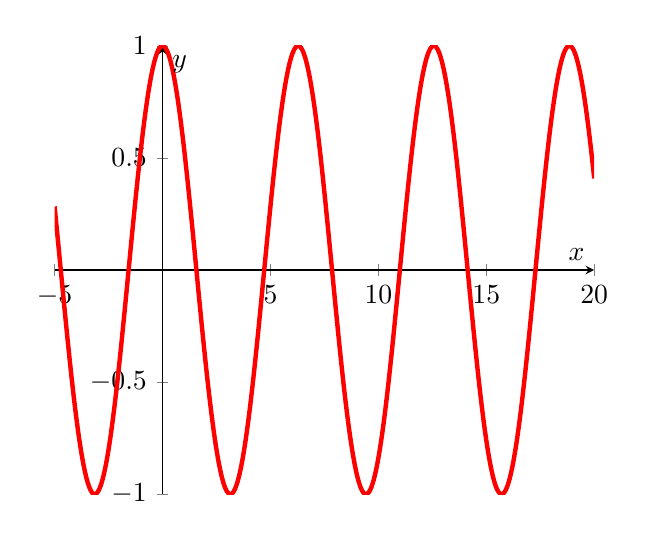
\begin{tikzpicture}
    \begin{axis}[
%    axis equal,
    samples=500,
    axis lines=middle,
    ylabel=$y$, 
    xlabel=$x$
    ]
    \addplot[domain=-5:20, black, ultra thick, color=red] {cos(deg(x))};
    \end{axis}
    \end{tikzpicture}
\end{center}
}

Bestudeer nu de eigenschappen van $\cos(ax+b)$ in Geogebra:


\begin{center}
    \geogebra{zwrge8pa}{400}{300}
\end{center}



% Uitgecommentarieerd: sage werkt niet correct in de KU Leuven setup
%  -> zie apart .tex bestand
\begin{comment}
\subsubsection{Ken je Sage al?}

In Sage kan je relatief eenvoudig de parametervergelijkingen van een cirkel bestuderen:

\begin{sageCell}
    var('s t')
    x(t) = 3*cos(t)
    y(t) = 3*sin(t)
    c(t) = (x(t),y(t))
    circle=parametric_plot(c(t),(t,0,2*pi),color="black")
    circle
\end{sageCell}

\pdfOnly{In de onlineversie kan je met deze code experimenteren. 
    
    Zie [één of andere ingewikkelde url] of [een qrcode]
}

\begin{onlineOnly}
    
    Pas de code aan, en druk op Evaluate!
    
    Nice, zoals ze zeggen ...
    
\begin{sageOutput}
    var('s t')
    x(t) = 3*cos(t)
    y(t) = 3*sin(t)
    c(t) = (x(t),y(t))
    circle=parametric_plot(c(t),(t,0,2*pi),color="black")
    circle
\end{sageOutput}
\end{onlineOnly}
\end{comment}

\section{Styling}
	De online versie kan gestyled worden door css files toe te voegen:
	\begin{itemize}
		\item \verb|global.css| in de root map van de repository: alle activities in de repository gebruiken deze styling
		\item \verb|xoursefilename.css| in de folder van xoursefilename.tex file: alle activities in de xourse gebruiken deze styling
		\item \verb|activityfilename.css| in de folder van de activityfilename.tex file: styling specifiek voor 1 activity.
	\end{itemize}
	De \verb|ximeraShowcase.css| file specifieert in dit geval dat de questions niet alleen links maar ook rechts een paarse balk hebben. 
    % niet het geval ...?

\subsection{Voorbeelden van het gebruik van environments}
\begin{definition}[Absolute waarde]\label{showcase:absolutewaarde}
	Voor een reëel getal $a\in\R$ definiëren we de \textit{absolute waarde} van $a$, genoteerd $|a|$, als
	\[
		|a| \perdef\displaystyle\ 
		          \left\{
			\begin{array}{rll  } 
				a  & \mbox{als} & a \geq 0 \\
				-a & \mbox{als} & a<0.
			\end{array}\right.
	\]
\end{definition}
\begin{remark}[Eigenschappen van de absolute waarde (met $a\in\R$)] \nl
		\begin{enumerate}
			\item Pas op: $|-a|= |a|$, maar \textsc{zeer zeker niet} $\xcancel{|-a|=a}$
			
			$|-a|=a$ is \textsc{fout} als $a<0$: als $a=-7$, dan is $|-a| = |-(-7)| \neq -7 = a$
			\item $|a^2 + 1| = a^2 + 1$, want $a^2+1$ is altijd positief.
			\item $|a^2 - 1| = ....$ \qquad(er is \textsc{geen} eenvoudige algemene formule zonder $|\cdot|$)
\end{enumerate}
\end{remark}
\begin{example}[Eenvoudige voorbeelden van absolute waarden] \nl 
	
\begin{xmmulticols}
    \begin{question}
        $|5|=5$ en $|-5|=5$
    \end{question}
    \begin{question}
        $|2 + 1| = |2| + | 1|\quad (=3)$
    \end{question}
    \begin{question}
        $|2 + (-1)| \neq |2| + | -1|$ (want $1\neq 3$)
    \end{question}
    \begin{question}
        $|(-3)^2| = |3^2| = 9\quad (=|-3^2| = |-9|) $
    \end{question}
    \begin{question}
        $|\sqrt{2}-1|=$\wordChoice{\choice[correct]{$\sqrt{2} - 1$}\choice{$1-\sqrt{2}$}}
    \end{question}
    \begin{question}
        $|1-\sqrt{2}| = $\wordChoice{\choice[correct]{$\sqrt{2} - 1$}\choice{$1-\sqrt{2}$}}
    \end{question}
    \begin{question}
        $|2-\sqrt{2}| = $\wordChoice{\choice{$\sqrt{2} - 2$}\choice[correct]{$2-\sqrt{2}$}}
    \end{question}
    \begin{question}
        $|\sqrt{2}-2| = $\wordChoice{\choice{$\sqrt{2} - 2$}\choice[correct]{$2-\sqrt{2}$}}
    \end{question}  
\end{xmmulticols}
\end{example}

Het gebruik van \verb|\begin{prompt}|: in de handout versie staat hieronder \textit{niets}

%\begin{prompt}  

%    want deze zin staat in een zogenaamde 'prompt' omgeving in \LaTeX, en die wordt \textit{niet} getoond in de handout versie, wel in de standaard pdf en online. 
    
%	Dit kan een alternatief zijn voor \verb|\begin{onlineOnly}|: voor zaken die enkel interactief relevant zijn,  zoals bijvoorbeeld, dat je geen derdemachtswortel kan ingeven online, en je dus ${}^\frac{1}{3}$ moet gebruiken.
    
%    In de standaard PDF is dit weergegeven als 'hidden tekst' (dus grijs in plaats van zwart).
    
%\end{prompt}


\end{document}
